\section{Methode}

Für die Bestimmung der Evapotranspiration werden die Lysimeter- und Meteodaten mit MATLAB prozessiert. Da die Meteodaten in UTC und die Lysimeterdaten in MEZ vorliegen, müssen die Datensätze zuerst an eine Zeit angepasst werden. Zudem müssen die Einheiten so angepasst werden, dass sie auf die jeweiligen Berechnungsformeln passen.

\subsection{FAO Penman-Monteith}

Die Penman-Monteith-Methode kombiniert die beiden Ansätze der Massenbilanz und der Energiebilanz. Alle in der Formel enthaltenen Parameter können entweder direkt gemessen oder dann aus meteorologischen Daten berechnet werden. Die Methode impliziert, dass der aerodynamische und der Oberflächenwiderstand von der Oberflächenbepflanzung abhängig sind [vgl.\,Abb.\,\ref{fig:widerstand}]. 

\begin{figure}[H]
\centering
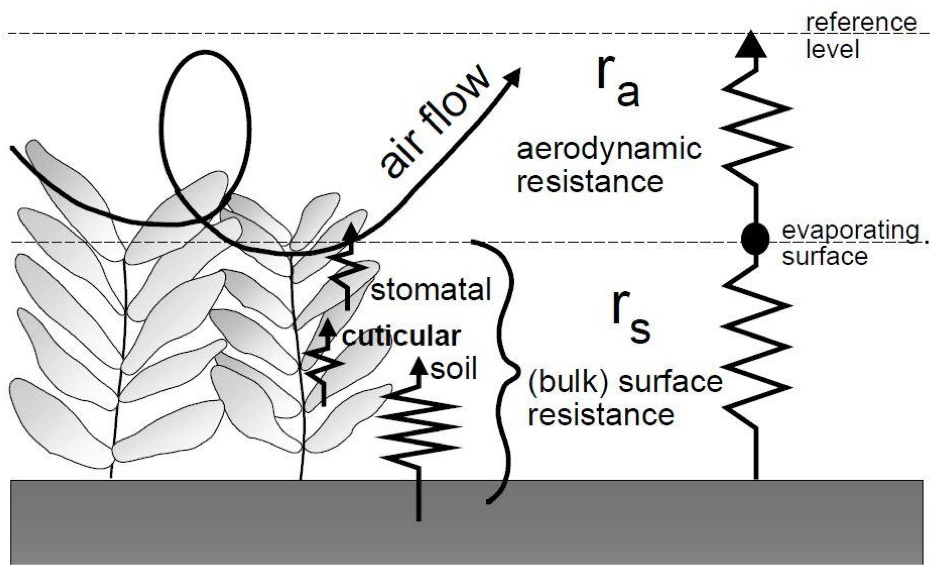
\includegraphics[width=0.8\textwidth]{figures/penman_widerstand.jpg}
\caption{Schematische Darstellung des aerodynamischen und des Oberflächenwiderstands in der Penman-Monteith-Methode}
\label{fig:widerstand}
\end{figure}

Der aerodynamische Widerstand beschreibt die Grösse, welche Wärme und Wasserdampf daran hindert , wegtransportiert zu werden. Diese hängt von der Windgeschwindigkeit und der Bodenrauigkeit ab. Der Oberflächenwiderstand beschreibt den Widerstand des Wasserdampfes, sich zwischen den transpirierenden Pflanzen und dem evaporierendem Boden zu bewegen. Dieser ist abhängig von Verhältnis der Blattfläche zur Bodenfläche und dem Stomatawiderstand eines gut bestrahlten Blattes. Unter Berücksichtigung dieser Einflüsse folgt die FAO\,Penman-Monteith-Formel für die Referenzfäche:

\begin{equation}
\label{eq:penman_ref}
ET_0=\frac{0.408\Delta \left(R_n-G\right)+\gamma \frac{900}{T+273}u_2\left(e_s-e_a\right)}{\Delta +\gamma\left(1+0.34u_2\right)}
\end{equation}
\begin{table}[H]
\centering
\begin{tabular}{ll}
$\mathrm{ET_0}$ & potentielle Referenzevapotranspiration $\mathrm{[mm/s]}$\\
$\mathrm{R_n}$ & Nettostrahlung $\mathrm{[W/m^2]}$ \\
$\mathrm{G}$ & Bodenwärmefluss $\mathrm{[W/m^2]}$\\
$\mathrm{\Delta}$ & Steigung der Sättigungsdampfdruckkurve $\mathrm{[kPa/^{\circ}C]}$\\
$\mathrm{\gamma}$ & Psychrometerkonstante $\mathrm{[kPa/^{\circ}C]}$\\
$\mathrm{T}$ & mittlere Temperatur in 2\,m Höhe $\mathrm{[^{\circ}C]}$\\
$\mathrm{u_2}$ & Windgeschwindigkeit in 2\,m Höhe $\mathrm{[m/s]}$\\
$\mathrm{e_s}$ & Sättigungsdampfdruck $\mathrm{[kPa]}$\\
$\mathrm{e_a}$ & aktueller Dampfdruck [kPa]\\
\end{tabular}
\end{table}

In den folgenden Berechnungen wird der Bodenwärmefluss allerdings vernachlässigt. Um die Evapotranspiration einer spezifischen Pflanze zu bestimmen, wird die Referenzevapotranspiration mit einem Pflanzenfaktor multipliziert. Es folgt daraus:

\begin{equation}
\label{eq:penman_spez}
ET_C=K_C*ET_0
\end{equation}
\begin{table}[H]
\centering
\begin{tabular}{ll}
$\mathrm{ET_0}$ & potentielle Referenzevapotranspiration $\mathrm{[mm/s]}$\\
$\mathrm{K_C}$ & Pflanzenfaktor [-]\\
$\mathrm{ET_C}$ & Evapotranspiration einer spezifischen Pflanze $\mathrm{[mm/s]}$\\\
\end{tabular}
\end{table}

Die Nettostrahlung $\mathrm{R_n}$ und die Temperatur T können aus den Meteodaten entnommen werden. Die übrigen Parameter müssen berechnet werden. Die FAO\,\cite{fao} gibt folgende Formeln:

\begin{description}
\item[Steigung der Sättigungsdampfdruckkurve]~
\begin{equation}
\label{eq:steigung}
\Delta=\frac{4098\left[0.6108*e^{\frac{17.27*T}{T+237.3}}\right]}{\left(T+237.3\right)^2}
\end{equation}
\begin{table}[H]
\centering
\begin{tabular}{ll}
$\mathrm{\Delta}$ & Steigung der Sättigungsdampfdruckkurve $\mathrm{[kPa/^{\circ}C]}$\\
T & Temperatur mittlere Temperatur in 2\,m Höhe $\mathrm{[^{\circ}C]}$\\
\end{tabular}
\end{table}


\end{description}

